\section{Funktionen }
	\subsection{Impulsfunktion - Dirac Delta Funktion \skript{34}}
		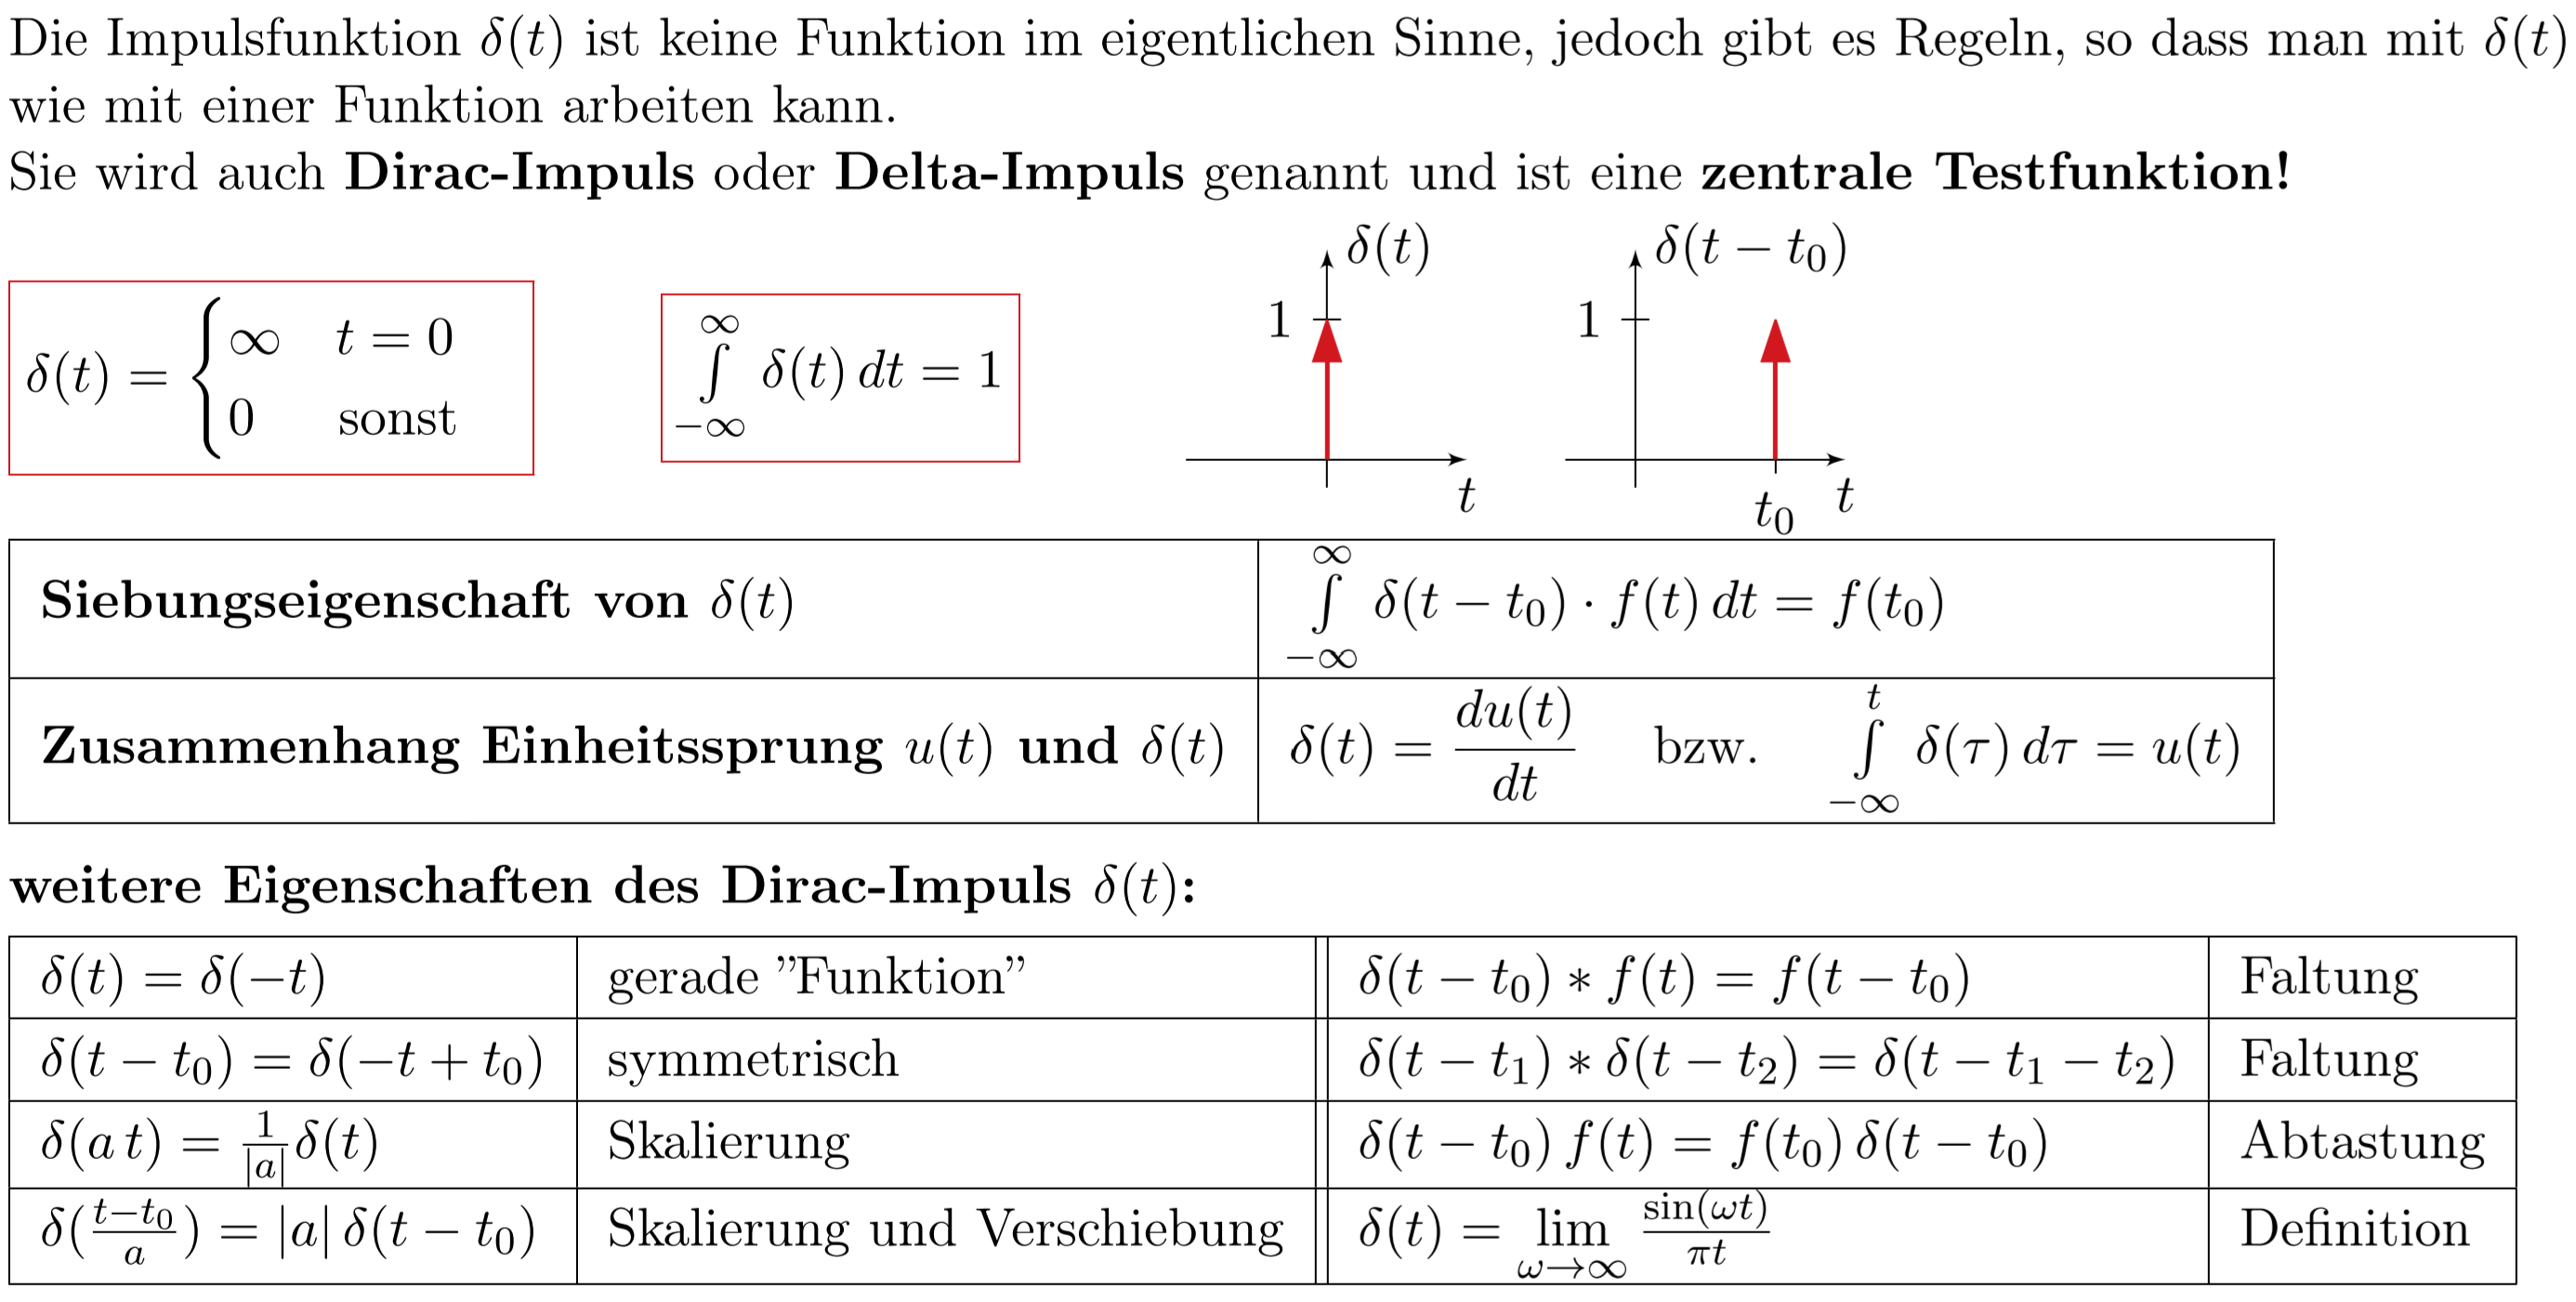
\includegraphics[width=0.95\textwidth]{./bilder/funktionen/impulsF.png}\\

        
        Bei einer Faltung mit einer $\delta\left(t\right)$ Funktion
        gilt: $f\left(t\right) \ast \delta\left(t\right) = f\left(t\right)$
	
	\subsubsection{Fouriertransformierte $\delta(t)$}
		$\delta(t) \; \laplace \; 1(\omega)$ \qquad
		$\delta(t-t_0) \; \laplace \; e^{-j\omega t_0}$ \qquad
		$1(t) \; \laplace \; 2\pi \delta(\omega)$



	\subsection{$\sigma$-Funktion, Schrittfunktion, unit-step}
		\begin{minipage}{0.2\textwidth}
			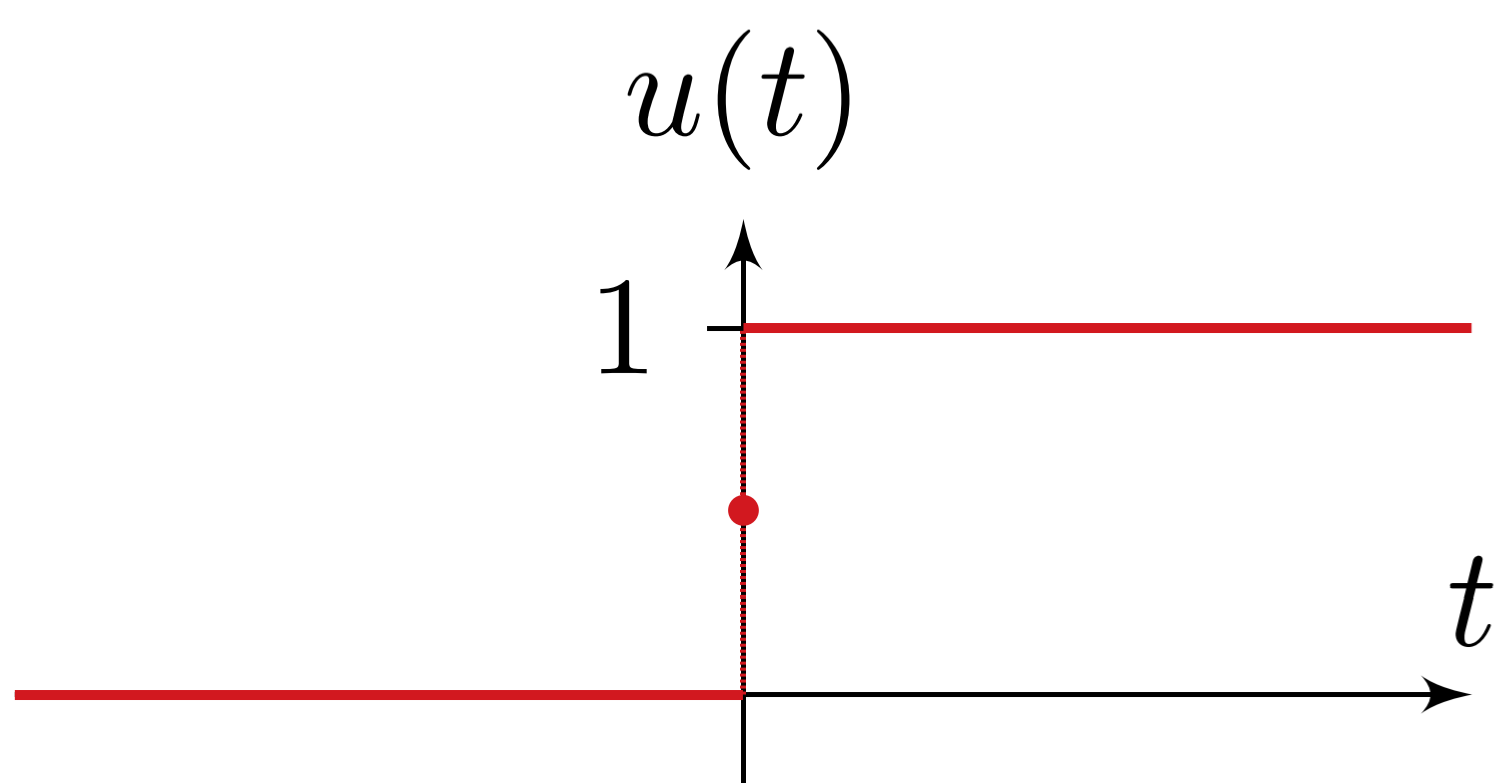
\includegraphics[width=\textwidth]{./bilder/funktionen/sprungF.png}
		\end{minipage}
		\qquad
		\begin{minipage}{0.45\textwidth}
			$u(t) = \sigma(t) =	\begin{cases}
			0 & \text{f\"ur } t < 0 \\
			\frac{1}{2} \text{(praxis)}  \text{ oder undef. (math.)} & \text{f\"ur } t = 0 \\
			1 & \text{f\"ur } t > 0
			\end{cases}$
		\end{minipage}
		\qquad
		\begin{minipage}{0.25\textwidth}						
			$\sigma(t) \; \laplace \; \frac{1}{j\omega} + \pi\delta(\omega) = \Sigma(\omega)$ \\
			\\
			$\frac{du(t)}{dt}=\delta(t)$\\
		\end{minipage}
	
	
	\subsection{Signumfunktion \skript{26}}
		\begin{minipage}{0.2\textwidth}
			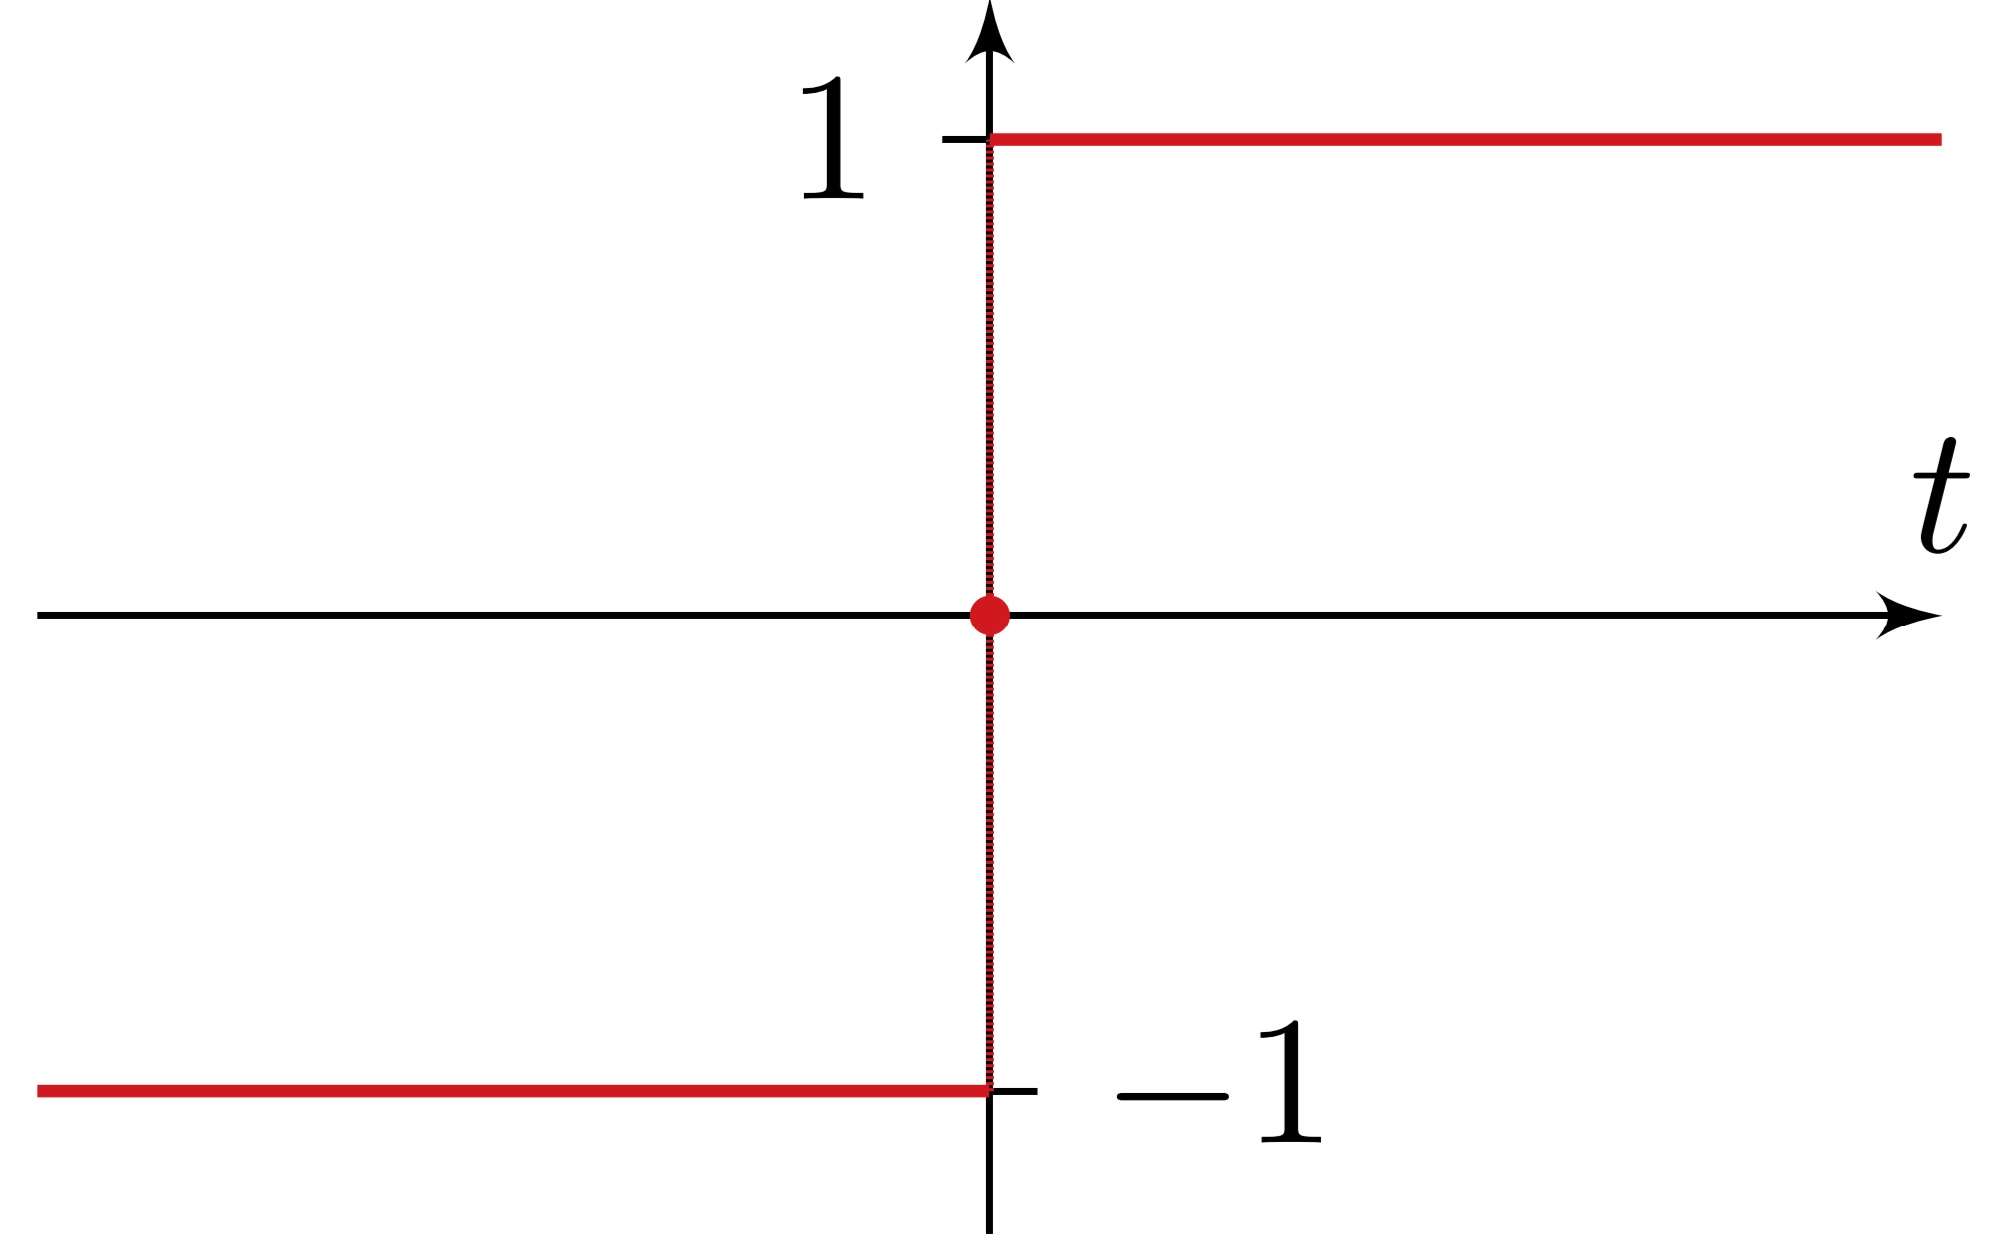
\includegraphics[width=\textwidth]{./bilder/funktionen/signF.png}
		\end{minipage}
		\qquad
		\begin{minipage}{0.45\textwidth}
			$sgn(t) = \begin{cases} 1 & \text{falls }t > 0 \\ -1 & \text{falls }t < 0 \end{cases}$
		\end{minipage}
		\qquad
		\begin{minipage}{0.25\textwidth}
            \begin{math}
                \begin{aligned}
                   sgn(t) \; &\laplace \; \frac{2}{j\omega}\\
                   \frac{1}{\pi t} \; &\laplace \; -j \cdot sgn(\omega)
                \end{aligned}
            \end{math}						
		\end{minipage}
	
	\subsection{Funktionen manipulieren}
		\includegraphics[width=0.8\textwidth]{./bilder/funktionen/SignalManip.png}	
	